\documentclass{cernatsnote}
\usepackage{physics}

\usepackage{tcolorbox}
\tcbuselibrary{skins}
\usepackage{lipsum}
\usepackage{mathtools}
\usepackage{amsfonts}
\usepackage[colorinlistoftodos]{todonotes}
\usepackage{placeins}
\usepackage{amsmath}
\usepackage{physics}
\usepackage{tcolorbox}
\tcbuselibrary{skins}
\usepackage{lipsum}
\usepackage{amsmath}
\usepackage[T1]{fontenc}
\usepackage{graphicx, subfigure}
\usepackage{fancyhdr}
\usepackage{lmodern}
\usepackage{color}
\usepackage{transparent}
\usepackage{amsfonts}
\usepackage{mathtools}
\usepackage{tikz}
\usetikzlibrary{positioning}
\usepackage{pgfplots}
\pgfplotsset{compat=1.10}
\usepackage{textcomp}
\usepackage{float}
\usepackage{adjustbox} % Used to constrain images to a maximum size 
\usepackage{color} % Allow colors to be defined
\usepackage{enumerate} % Needed for markdown enumerations to work
\usepackage{geometry} % Used to adjust the document margins
\usepackage{amsmath} % Equations
\usepackage{amssymb}
\usepackage{fancyvrb} % verbatim replacement that allows latex
\usepackage{grffile} % extends the file name processing of package graphics 
                         % to support a larger range 
    % The hyperref package gives us a pdf with properly built
    % internal navigation ('pdf bookmarks' for the table of contents,
    % internal cross-reference links, web links for URLs, etc.)
\usepackage{hyperref}
\usepackage{longtable} % longtable support required by pandoc >1.10
\usepackage{tabularx}
\usepackage{epigraph}
\usepackage{quotchap}
\usepackage{lscape}
\usepackage{enumerate}
\usepackage{xpatch}
\usepackage{titletoc}
\usepackage{float}	
\usepackage{xparse}
\NewDocumentCommand{\DIV}{om}{%
  \IfValueT{#1}{\setcounter{#2}{\numexpr#1-1\relax}}%
  \csname #2\endcsname
}

%\renewcommand{\thesubsection}{\thesection.\alph{subsection}}


\title{Computational Physics – Exercise 1}
\author{Pugazharasu Anancia Devaneyan, Rishi Kumar Senthil Kumar}
\email{\href{pugs@uni-bonn.de}{pugs@uni-bonn.de}, \href{s6risent@uni-bonn.de}{s6risent@uni-bonn.de}}
\date{\today}

\begin{document}
\maketitle

%\begin{abstract}
%This document summarizes ideas from Group theory and representation theory that are vital for the upcoming seminar.
%\end{abstract}
%\\ \\ \\ 

%\begingroup
%\color{black}
%\tableofcontents
%\endgroup

%\section*{Test}
%\section*{Simulation of the 1-D Ising model}
\section{What is $J$?}
For the 1-D Ising Hamiltonian,
\begin{equation}
    \mathcal{H}(s)=-J \sum_{\langle x, y\rangle} s_x s_y-h \sum_x s_x
\end{equation}
Where $\langle x, y\rangle$ denotes a sum over the nearest spins and $h$ is the external coupling. $J$ is a coupling constant that models the interaction between neighbouring spins. For $J>0$, the similar nearest neighbour pairs are favoured as this minimizes the total energy. In this context of magnets, this corresponds to having ferromagnetic order (see figure \ref{fig:ferro}) \cite{thijssen}.
\begin{figure}[H]
    \centering
    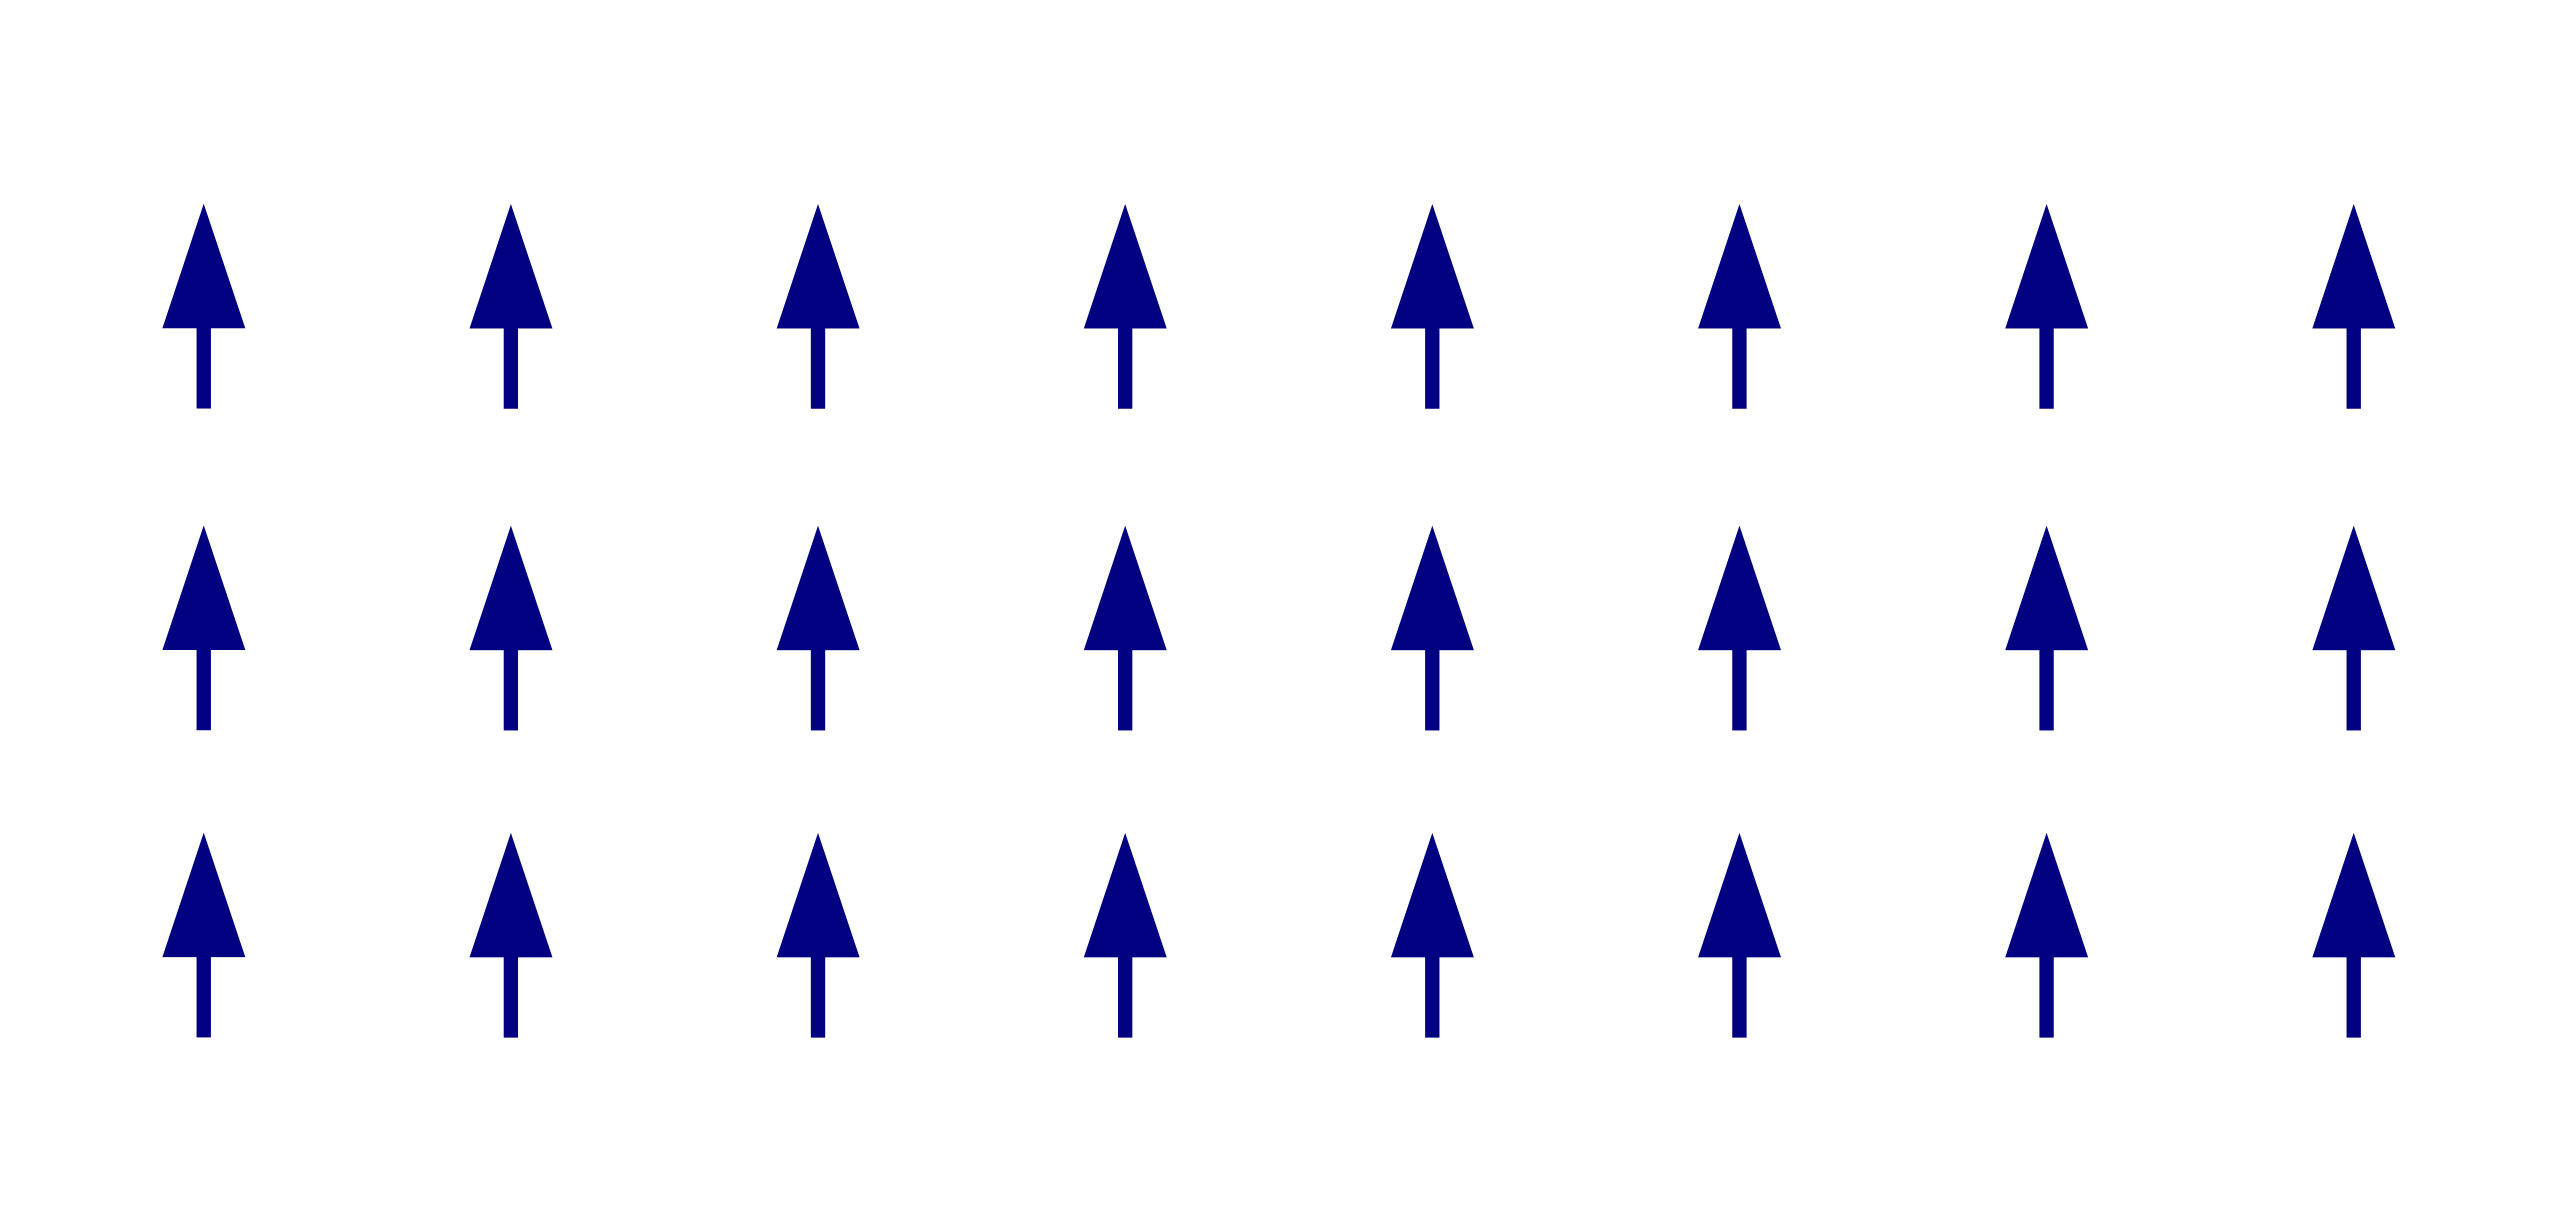
\includegraphics[scale=0.1]{images/Ferromagnetic_ordering.svg.png}
    \caption{Ferromagnetic ordering in $d=2$. Taken from \cite{ferro}}
    \label{fig:ferro}
\end{figure}
For $J<0$, opposite nearest neighbour pairs are favoured. In this context of magnets, this corresponds to having anti-ferromagnetic order (see figure \ref{fig:anti_ferro}).
\begin{figure}[H]
    \centering
    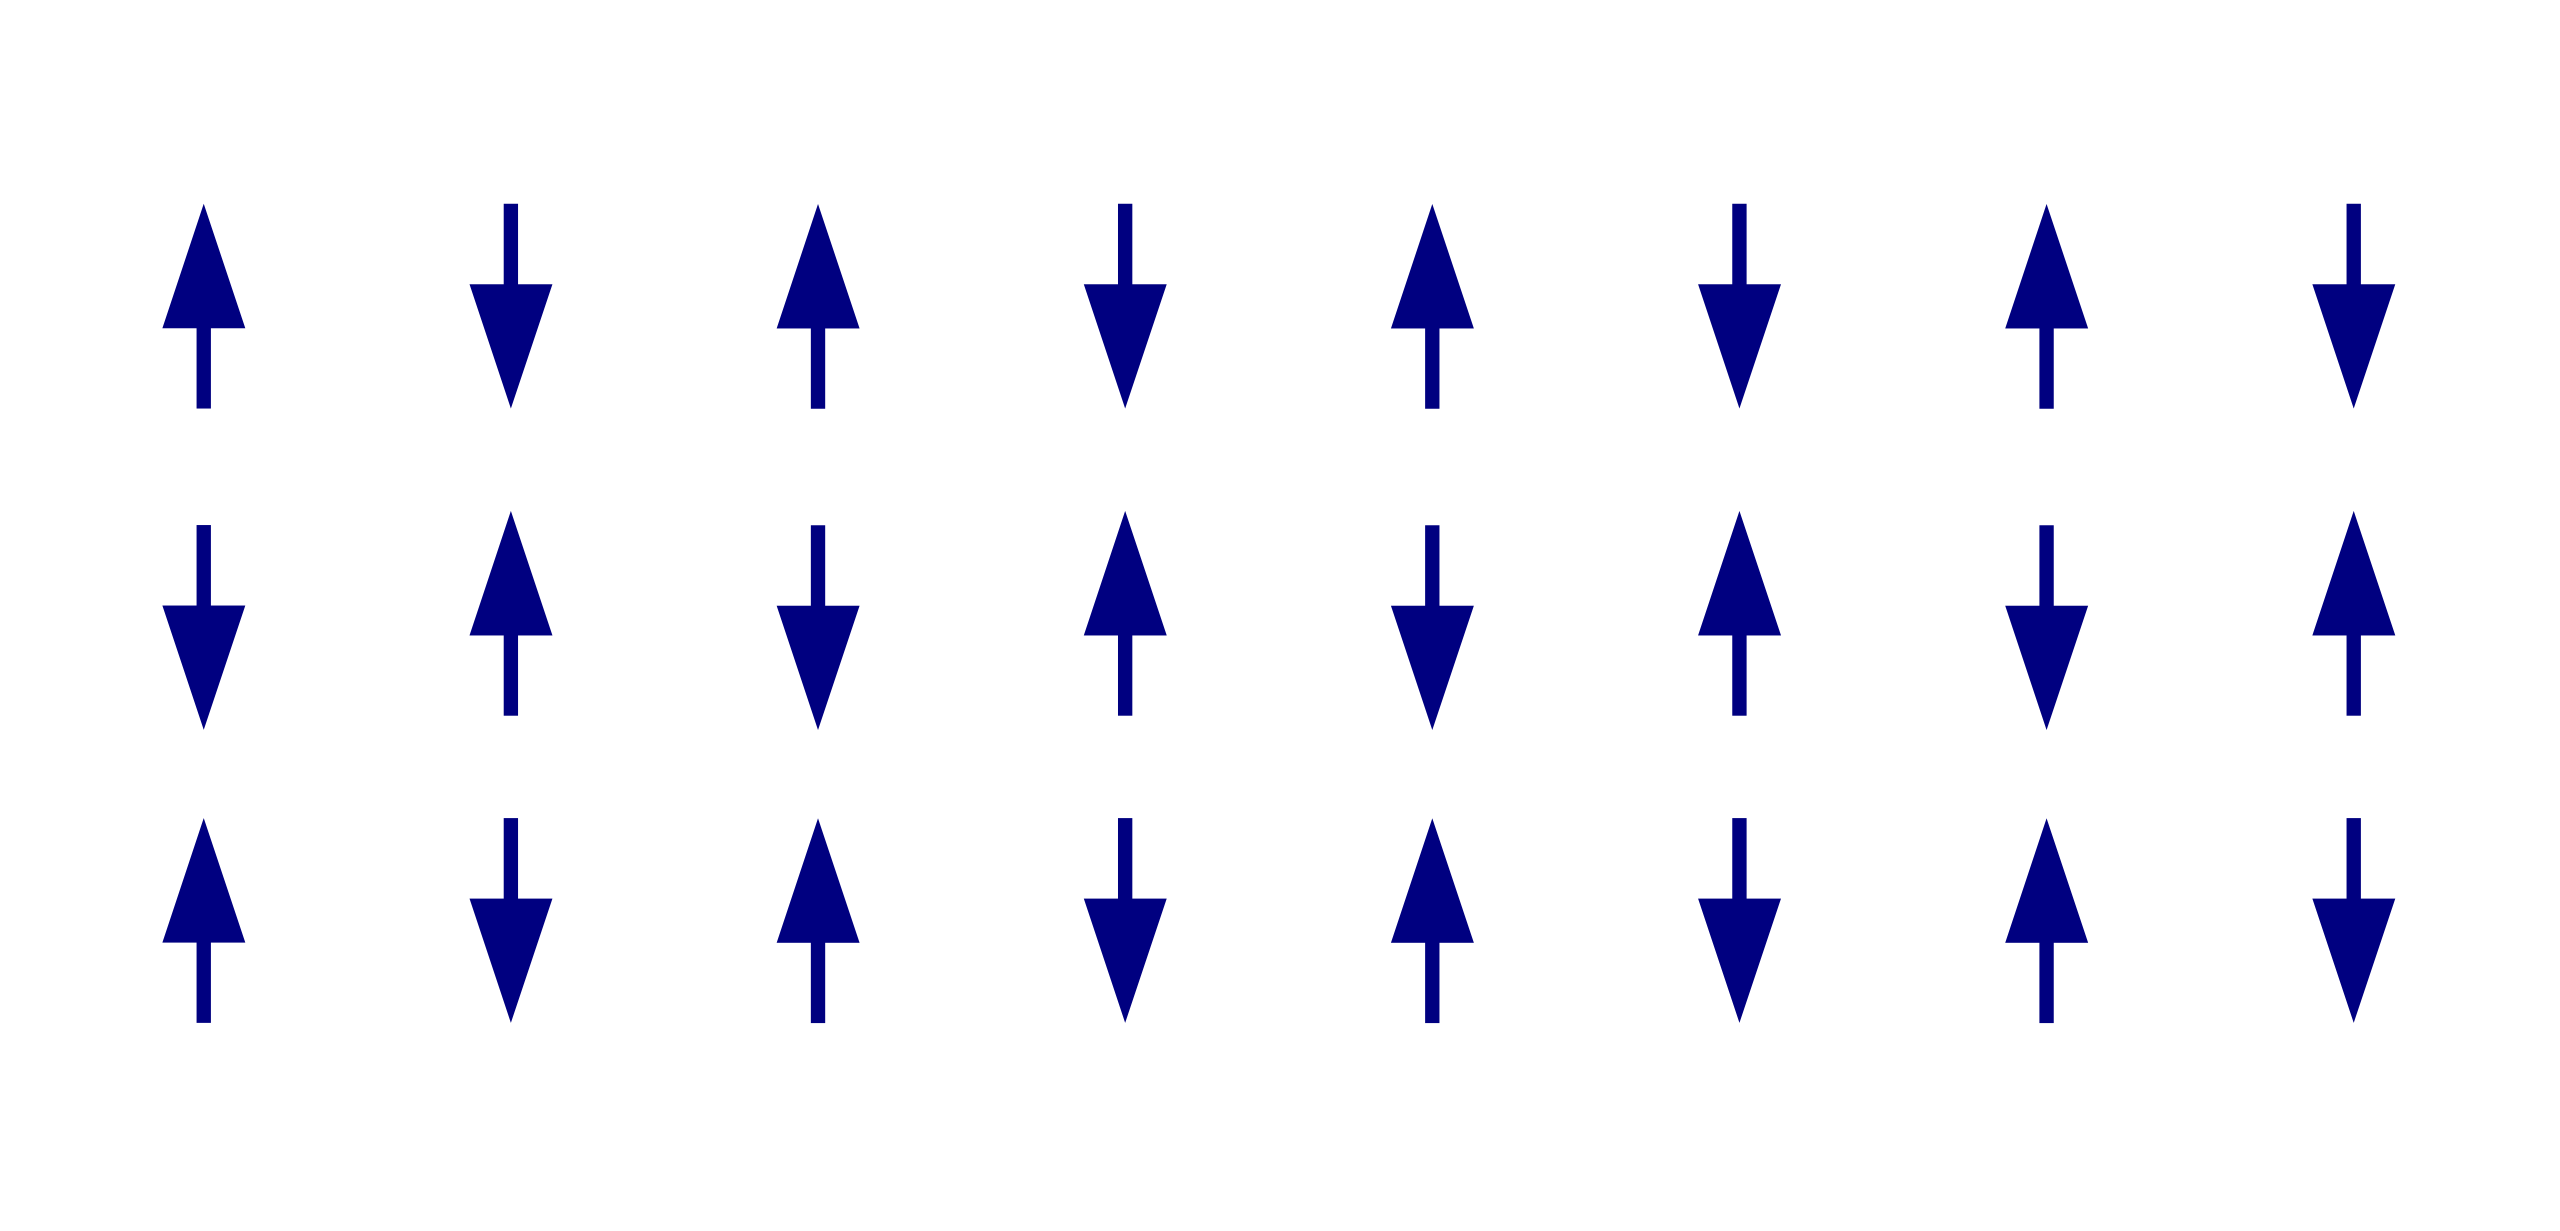
\includegraphics[scale=0.1]{images/Antiferromagnetic_ordering.svg.png}
    \caption{Antiferromagnetic ordering in $d=2$. Taken from \cite{anti}}
    \label{fig:anti_ferro}
\end{figure}

\section{Periodic boundary conditions}
Having periodic boundary conditions implies that all sites have the same number of  nearest neighbours \cite{newman}.
\section{Simulating the Ising model in $d=1$}
The average magnetization is given by:
\begin{equation}
    \expval{m} = \frac{T}{N} \frac{\partial}{\partial h}\ln{Z}
\end{equation}
Where the partition function $Z$ is given by,
\begin{equation}
    Z = \lambda_{+}^{N} + \lambda_{-}^{N}
\end{equation}
for
\begin{equation}
    \lambda_{\pm} = \mathrm{e}^{\frac{J}{T}}\left(\cosh \left(\frac{h}{T}\right) \pm \sqrt{\sinh \left(\frac{h}{T}\right)^2+\mathrm{e}^{-4 \frac{J}{T}}}\right)
\end{equation}
In this problem the relevant dimensionless ratios are as follows:
\begin{itemize}
    \item $\frac{J}{T}$
    \item $\frac{h}{T}$
\end{itemize}
In order to calculate the average magnetization numerically, we use the formula
\begin{equation}
   \expval{m}  = \frac{1}{N} \sum_{i}S_{i}
\end{equation}
We shall now simulate the Ising model in $d=1$, the python code for that can be found at \cite{github}. 
\begin{figure}[H]
    \centering
    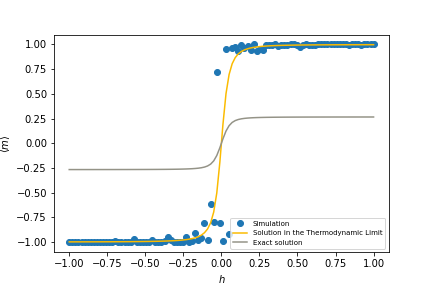
\includegraphics[scale =0.7]{images/m_v_h.png}
    \caption{A plot of the $\langle m \rangle$ versus external field $h$ for a fixed $J = 1$, $T = 0.75$ and $N = 20$.}
    \label{fig:h_v_m}
\end{figure}
\begin{figure}[H]
    \centering
    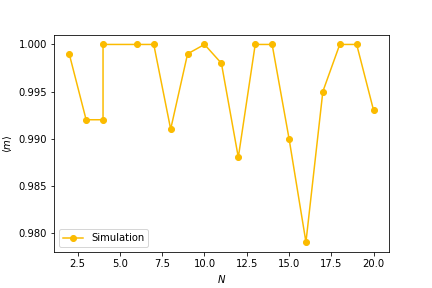
\includegraphics[scale =0.7]{images/m_v_n.png}
    \caption{A plot of the $\langle m \rangle$ versus external field $N$ for a fixed $J = 1$, $T = 0.75$ and $h = 0.5$.}
    \label{fig:N_v_m}
\end{figure}
\begin{figure}[H]
    \centering
    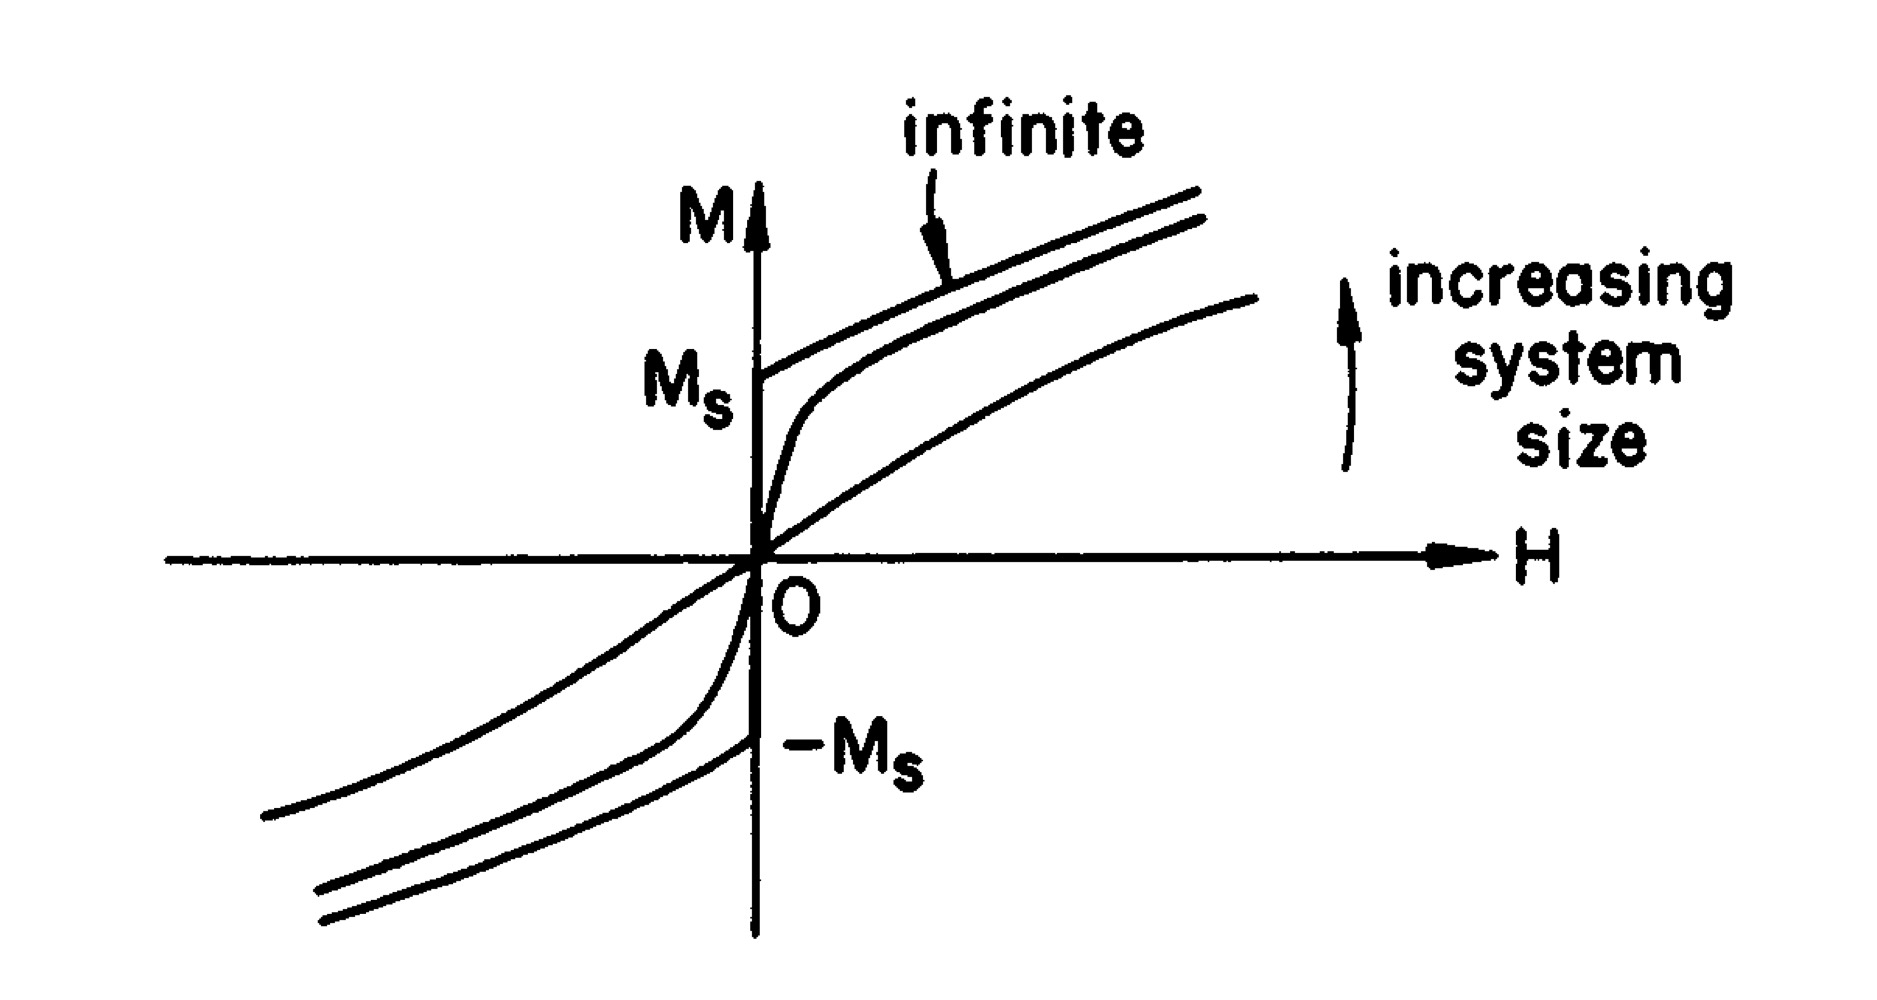
\includegraphics[scale=0.15]{images/mag.jpeg}
    \caption{A plot of magnetisation $M$ versus the external coupling parameter $H$. Taken from \cite{goldenfeld}.}
    \label{fig:m_golden}
\end{figure}
Numerically we were able to approximate $\langle m \rangle$ close enough to the value we observe at the thermodynamic limit as shown in figure \ref{fig:h_v_m}. We can compare this to a plot from the literature in figure \ref{fig:m_golden}, we find these to be in close agreement. We find that the value of $\expval{m}$ is constrained heavily by the couplings $h$ and $J$, however it does it does vary a little depending on the number of sites for $d=1$ i.e. if it is even or odd and so on (see figure \ref{fig:N_v_m}).

We computed the error for simulation via the residual standard deviation, which came to about $0.0004$. 
\bibliographystyle{abbrv}
\bibliography{Bibliography.bib}
\end{document}